\section{Proposed Methodology: \ours}
\label{sec:method}

%
\paragraph{Model preliminaries.} We first review the meta-architecture of M2F \cite{cheng2021mask2former} upon which {\ours} is based, along with the notation. This class of models contains
\begin{itemize}
    \item a \emph{backbone} $\bbF(\cdot)$ which takes the $\idx$-th image $\inImg\superIdx$ as input to generate multi-scale feature maps $\bbF(\inImg\superIdx)$, represented as ${\feature_1, \feature_2, \feature_3, \feature_4}$. These multi-scale feature maps correspond to spatial resolutions typically set at $\nicefrac{1}{32}$, $\nicefrac{1}{16}$, $\nicefrac{1}{8}$, and $\nicefrac{1}{4}$ of the original image size, respectively.
    \item a \emph{transformer encoder} (called the ``pixel decoder'' \cite{cheng2021mask2former}), which is composed of multiple layers of transformer encoders. The function of this module is to generate rich token representation from $\{\feature_1, \feature_2, \feature_3\}$ and generate per-pixel embeddings from $\feature_4$. Each layer in the transformer encoder, denoted as $\pdF_\Glayer(\cdot)$ (where $\Glayer\in\{1,2,\dots,\NGlayer\}$) is successively applied to $\bbF(\inImg\superIdx)$, with $\pdF_\NGlayer(\cdot)$ being the last layer in the transformer encoder. 
    \item a \emph{transformer decoder} (along with a segmentation head) that takes two inputs: the output of the transformer encoder and the object queries. The object queries are decoded to output a binary mask along with the corresponding class label. 
\end{itemize}
For brevity, we collectively refer to the operations in the transformer decoder and segmentation head together as $\headF(\cdot)$. Thus, the output of the meta-architecture with $K$ encoder layers (a predicted mask $\outMF_\NGlayer\superIdx$ and corresponding label $\tilde{\ell}_\NGlayer\superIdx$) can be written as 
\begin{equation}
    \{\outMF_\NGlayer\superIdx, \tilde{\ell}_\NGlayer\superIdx\} = h\circ f_\NGlayer\circ\cdots\circ f_2\circ f_1\circ b(\inImg\superIdx)\,.
\end{equation}
Here, the operation $\circ$ represents function composition, \eg, $g\circ f(x) = g(f(x))$ and subscript denotes output predicted using $K$ encoder layers. With $\{\gtseg\superIdx, \ell\superIdx\}$ as the pair of ground truth segmentation map and corresponding label of image $\inImg\superIdx$, the final loss \cite{cheng2021mask2former} is computed as
\begin{align}
    \loss_\NGlayer = \lambda_{\text{mask}}\loss_{\text{mask}}(\outMF_\NGlayer\superIdx, \gtseg\superIdx) + \lambda_{\text{class}}\loss_{\text{class}}(\tilde{\ell}_\NGlayer\superIdx, \ell\superIdx )\,,
    \label{eq:orig_loss}
\end{align}
where $\loss_{\text{mask}}(\cdot,\cdot)$ is a binary mask loss and $\loss_{\text{class}}(\cdot,\cdot)$ is the corresponding classification loss. $\lambda_{\text{mask}}$ and $\lambda_{\text{class}}$ represent the associated loss weights.
%
\paragraph{Method motivation.} Our motivation stems from the observation that layers within the transformer encoder of M2F exhibit non-uniform contributions to Panoptic Quality (PQ) \cite{kirillov2019panoptic}, as discussed in \Secref{sec:intro}. This prompts us to question the necessity of all $K=6$ layers for every image and target minimizing layer usage according to the user's computational constraints while ensuring that overall performance remains within acceptable bounds. Hence, we adopt an adaptive early exiting approach driven by three critical components:
\begin{enumerate}
    \item \emph{Model suitability for early exiting.} Traditional early exiting techniques \cite{tang2023you, xu2023lgvit, liu2021mevt, wang2022single, jiang2023multi, yang2023exploiting, valade2024eero, tang2023need, zhang2023adaptive} often face challenges in maintaining satisfactory performance levels at potential exit points throughout the neural network. We recognize the importance of a model architecture that not only allows for early exiting but also ensures that the performance remains consistently high. Therefore, we aim to develop a model that not only permits early exits but also for which the accuracy steadily improves as the network delves deeper into its architecture. By prioritizing this aspect, we seek to establish a framework where early exiting does not compromise the overall performance of the model.
    %
    \item \emph{Efficient and effective gating network for optimal exit decision making.} The efficacy of an early exiting strategy heavily depends on the ability to make informed exit decisions. A gating network must strike a delicate balance, minimizing computational overhead while effectively identifying components that can be bypassed without compromising accuracy. Our objective is to design a lightweight yet powerful gating mechanism capable of discerning optimal exit points within the model architecture.
    %
    \item \emph{Dynamic control mechanism for cost-performance trade-off.} We require a mechanism with the ability to adaptively regulate the balance between computational cost and performance according to user-defined priorities. Such a mechanism empowers the model to exit at the optimal layer based on specific needs and desired outcomes, ensuring efficient resource allocation and maximizing utility in various application scenarios, particularly in resource-constrained environments like edge computing or real-time applications.
\end{enumerate}

Driven by these considerations, {\ours} offers a novel training process that enables an adaptive early exiting mechanism designed to bolster computational efficiency while preserving satisfactory model accuracy. For better understanding, we'll begin with a general overview of model training and inference before diving into the specific details of our training process. 
%
\begin{figure*}[!t]
  \centering
  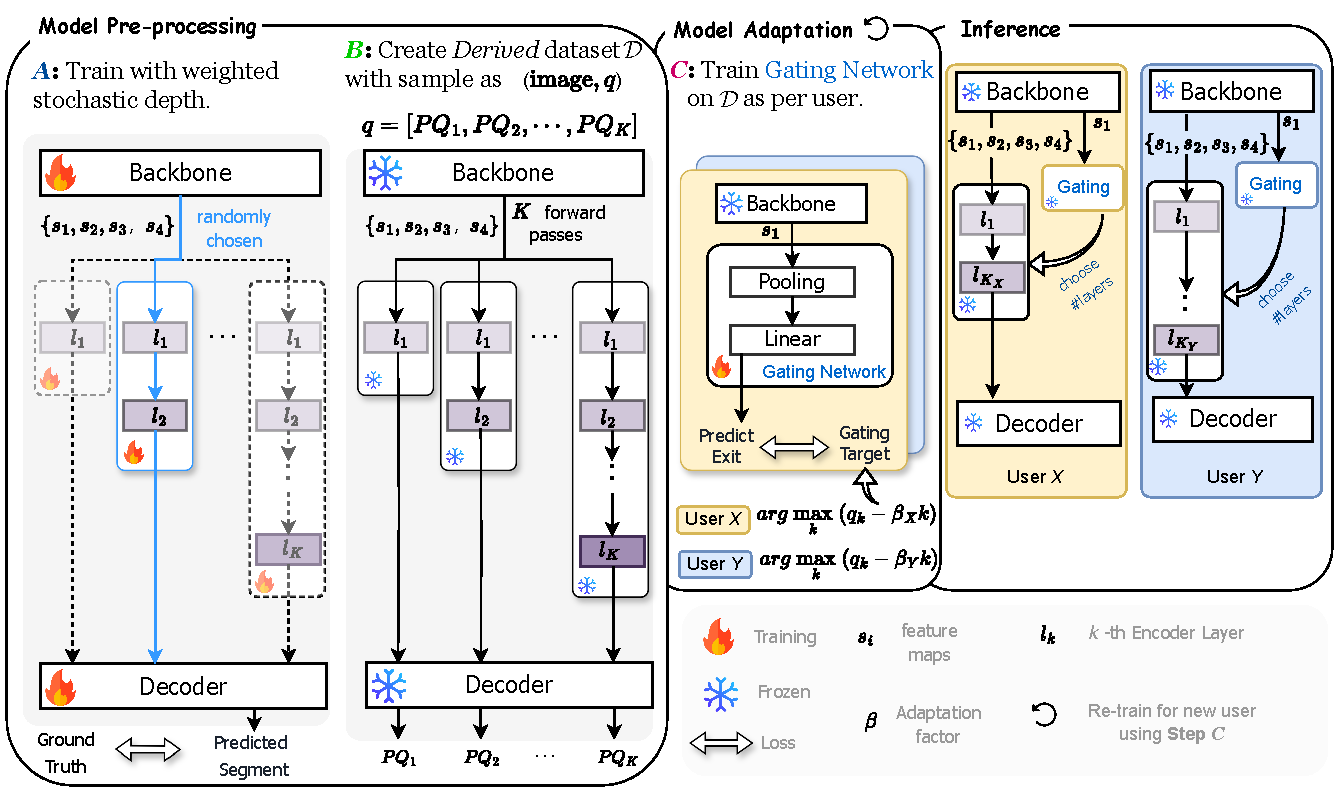
\includegraphics[trim={0 0 1.5em 0},width=\textwidth]{figures/images/main_framework.pdf}
  \caption{\textbf{{\ours} framework.} During the \textit{model pre-processing} phase, we train the model to exit stochastically at $\NGlayer$ potential exits using Step \stepA.  This is followed by Step \stepB, where we use this model to perform inference on the training images at each exit to create a dataset $\train$. In the \textit{model adaptation} phase, we perform Step \stepC to establish a gating target based on the computational budget and train a lightweight gating network. During \textit{inference}, the network adheres to the gating network's output and exits at its designated output layer.}
  \label{fig:main_framework} 
\end{figure*}
\paragraph{Training and Inference overview.} As shown in \Figref{fig:main_framework}, the training phase of {\ours} involves following three main steps: 
\begin{enumerate}[label={$\bullet$}, leftmargin=*]
    \item Step \stepA: Train parent model for early exit via the transformer encoder.
    %
    \item Step \stepB: Derive a dataset (which we call the Derived dataset) from the dynamic model obtained in Step \stepA.
    %
    \item Step \stepC: Train the \textit{Gating Network} to learn optimal exit points in the encoder tailored to users' requirements.
\end{enumerate}
We refer to Step \stepA and \stepB together as \textit{model pre-processing} and Step \stepC as \textit{model adaptation}. The former is required only once, whereas the latter is repeated as per user requirements. All these steps use the training data subset. 

During inference, the gating network guides the parent model by selecting the optimal exit point based on features extracted from the backbone with just one forward pass for final predictions.
%
\subsection{Step \stepA: Training the Model with Weighted Stochastic Depth}
\label{sec:SDwithP}
In this step, we enable the model to allow exiting at the encoder. To maintain consistently high performance at each exit point, we input each stochastic depth's output to a shared transformer decoder. We then apply \Eqref{eq:orig_loss} to compute the loss $\loss_\Glayer$ for each exit point $\Glayer$. However, we observe that direct training in this fashion does not encourage the model to use fewer layers to extract and prioritize informative representations, as shown in \Tabref{tab:loss}. To address this, we introduce a set of coefficients $\lossCoef_\Glayer$ to emphasize the quality of representations at later layers more, enabling earlier layers to also concentrate on producing effective intermediate representations. As the layer depth increases, the corresponding coefficient $\lossCoef_\Glayer$ grows, ensuring a progressively stricter standard for feature quality. The new loss function is then expressed as
\begin{equation}
    \label{eq:loss}
    \loss_{\text{total}} = \frac{1}{N}\sum_\idx^N\sum_{\Glayer}^\NGlayer \lossCoef_\Glayer\loss_\Glayer,\,\,{\text{where}}\ \forall \Glayer<\Glayer', \lossCoef_\Glayer<\lossCoef_{\Glayer'}\,,
\end{equation}
where $N$ is the number of images in the training set, and $\loss_\Glayer$ is from \Eqref{eq:orig_loss}.
\begin{wrapfigure}[18]{R}{0.45\textwidth}
    \centering
    \vskip-2em
    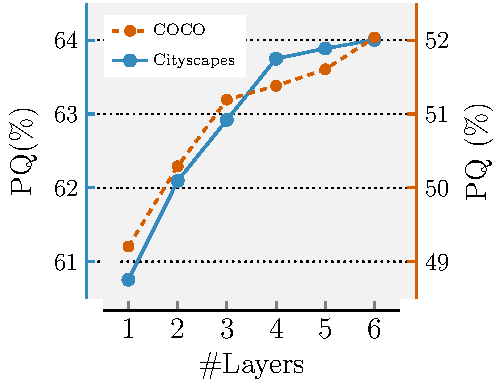
\includegraphics[width=0.45\textwidth]{figures/images/PQ_vs_layer_train_set.pdf}
    \caption{\textbf{Intuition for} \Eqref{eq:utility_func}. This figure shows that prioritizing PQ would need more encoder layers, and conversely, prioritizing lesser layers would result in poorer PQ. (Backbone: SWIN-T; training set).}
    \label{fig:PQ_vs_layers}
\end{wrapfigure}
%
\subsection{Step \stepB: Deriving the Gating Network Training Dataset}
To facilitate informed exit decisions during inference, our approach is to train a gating network to learn optimal exit strategies. In this step, we facilitate this gating network training by first deriving an intermediate dataset. 

To this end, we record the performance of the pre-trained stochastic depth model (obtained from Step \stepA) at all potential exit points for each image within the training dataset and create a \textit{Derived} dataset $\train$. Specifically, we associate the $\idx$-th input image $\inImg\superIdx$ with a vector $\pqv\superIdx$ of length $\NGlayer$. Each element $\evq_\Glayer\superIdx$ of $\pqv\superIdx$ represents the predicted panoptic quality \cite{kirillov2019panoptic} upon exiting at the encoder layer $\Glayer$. Hence, each sample of $\train$ can be represented as $ (\inImg\superIdx, \pqv\superIdx) \in \train$.
%
\subsection{Step \stepC: Training for Gating Network}
\label{sec:gating}
In this step, we train the gating network on dataset $\train$ (obtained from Step \stepB) to self-select the number of encoder layers based on the input image. Ideally, this module should allow exiting at the encoder layer which would result in the highest quality segmentation map. With this in mind, we first establish the target exit for the gating network. Note that the panoptic quality generally increases with increasing encoder layers (see \Figref{fig:PQ_vs_layers}). However, we would like the gating network to prioritize increasing the panoptic quality while also reducing the number of layers (to reduce the overall computations).  
Consequently, we introduce a utility function expressed as the linear combination of segmentation quality and the depth of the network. This function is formulated as
\begin{equation}
    \uF(\Glayer) = q_\Glayer\superIdx - \GPRatio\Glayer\,,
    \label{eq:utility_func}
\end{equation}
where $\GPRatio$ serves as an \textit{adaptation factor} governing the trade-off between segmentation quality and computational cost. Clearly, a higher value of $\GPRatio$ signifies a greater emphasis on efficiency over segmentation quality. Using \Eqref{eq:utility_func}, we determine a target exit point $\tgtIdx$ for each image $\inImg\superIdx$ using 
\begin{equation}
    \label{eq:target}
    \tgtIdx = \argmax_\Glayer (\uF(\Glayer))\,.
\end{equation}
With a target designated for each image using \Eqref{eq:target}, the gating decision can be approached as a straightforward classification problem. The gating architecture consists of a pooling operation $\vz(\cdot)$ on the token length dimension followed by a linear layer with weights $\mW$. Its output logits can be represented as 
\begin{align}
    \label{eq:gating}
    \Goutput\superIdx &= \mW \vz(\feature_1\superIdx)\,.
\end{align}
In consideration of having minimal impact on the computations due to the gating network, we use the output of the lowest resolution feature map $\feature_1$ as input to the pooling operation. To optimize the gating network, we use the standard cross-entropy loss between the output logits $\Goutput\superIdx$ and the one-hot version of target exit $\tgtIdx$ as our training objective. During inference, the gating network identifies the layer with the highest predicted logits, \ie, $\argmax_\Glayer(g_\Glayer\superIdx)$, as the optimal exit layer for image $\inImg\superIdx$. Note that while there can be more complex choices for the gating network, our simple linear layer in \Eqref{eq:gating} works well in our experiments.
%
\paragraph{Saving training costs through Step \stepC.}
 {\ours} presents a distinct advantage in terms of its adaptability to varying computational constraints. In scenarios where a smaller model is desired, {\ours} necessitates training solely the gating network (\ie, repeat Step \stepC). Assuming that the computational load is proportional to the depth of the network, \Eqref{eq:utility_func} enables us to weigh the performance gain against the computational overhead for each exit layer. We achieve this by setting the total number of layers $\NGlayer$ to a smaller number depending on user preferences. For instance, as illustrated in \Figref{fig:main_framework}, User $X$ preferring a smaller model compared to User $Y$ may opt for a smaller $\NGlayer$, \ie, $\NGlayer_X<\NGlayer_Y$. Then, given the importance of segmentation quality, we choose $\beta$. With these two variables set in \Eqref{eq:target}, we train the gating network. This capability shows that {\ours} is versatile and resource-efficient as it adapts to diverse needs and optimizes allocations.
%
\subsection{Inference}
In the inference phase, the gating network guides the parent model toward an optimal exit point tailored to each input image. Similar to the training phase, the gating mechanism receives low-resolution features from the backbone and produces a vector of length $\NGlayer$ for each image. The value of $\NGlayer$ remains consistent with that determined in Step \stepC. Subsequently, the gating network identifies the layer with the highest predicted logits as the optimal exit layer for each image. The parent model adheres to this decision, exiting at the determined layer, and subsequently progresses through the subsequent components to make the final prediction. This dynamic process ensures that the model adaptively selects the most optimal layer for exit during inference, enhancing its efficiency in handling diverse input data.